% !TEX TS-program = pdflatex
% !TEX encoding = UTF-8 Unicode

% This is a simple template for a LaTeX document using the "article" class.
% See "book", "report", "letter" for other types of document.

\documentclass[11pt]{article} % use larger type; default would be 10pt

\usepackage[utf8]{inputenc} % set input encoding (not needed with XeLaTeX)

%%% Examples of Article customizations
% These packages are optional, depending whether you want the features they provide.
% See the LaTeX Companion or other references for full information.

%%% PAGE DIMENSIONS
\usepackage{geometry} % to change the page dimensions
\geometry{a4paper} % or letterpaper (US) or a5paper or....
\geometry{margin=1in} % for example, change the margins to 2 inches all round
% \geometry{landscape} % set up the page for landscape
%   read geometry.pdf for detailed page layout information

   \usepackage[pdftex]{graphicx}
  % declare the path(s) where your graphic files are
   \graphicspath{{./figures/}}
  % and their extensions so you won't have to specify these with
  % every instance of \includegraphics
   \DeclareGraphicsExtensions{.pdf, .png}
% \usepackage[parfill]{parskip} % Activate to begin paragraphs with an empty line rather than an indent

%%% PACKAGES
\usepackage{booktabs} % for much better looking tables
\usepackage{array} % for better arrays (eg matrices) in maths
\usepackage{paralist} % very flexible & customisable lists (eg. enumerate/itemize, etc.)
\usepackage{verbatim} % adds environment for commenting out blocks of text & for better verbatim
\usepackage{subfig} % make it possible to include more than one captioned figure/table in a single float
% These packages are all incorporated in the memoir class to one degree or another...

%%% HEADERS & FOOTERS
\usepackage{fancyhdr} % This should be set AFTER setting up the page geometry
\pagestyle{fancy} % options: empty , plain , fancy
\renewcommand{\headrulewidth}{0pt} % customise the layout...
\lhead{}\chead{}\rhead{}
\lfoot{}\cfoot{\thepage}\rfoot{}

%%% SECTION TITLE APPEARANCE
\usepackage{sectsty}
\allsectionsfont{\sffamily\mdseries\upshape} % (See the fntguide.pdf for font help)
% (This matches ConTeXt defaults)

%%% ToC (table of contents) APPEARANCE
\usepackage[nottoc,notlof,notlot]{tocbibind} % Put the bibliography in the ToC
\usepackage[titles,subfigure]{tocloft} % Alter the style of the Table of Contents
\renewcommand{\cftsecfont}{\rmfamily\mdseries\upshape}
\renewcommand{\cftsecpagefont}{\rmfamily\mdseries\upshape} % No bold!

%%% END Article customizations

%%% The "real" document content comes below...

\title{Getting Started Guide of UnitFL}
%\author{Nan Wang}
\date{} % Activate to display a given date or no date (if empty),
         % otherwise the current date is printed 

\begin{document}
\maketitle

\section{Overview}

UnitFL is unit testing extension of Visual Studio. It has three main functions.
\begin{itemize}
\item{NUnit 3.0 Testing Adapter} \\
UnitFL implements a NUnit 3.0 testing adapter. You can write unit tests with NUnit 3.0 and run those tests in Test Explorer.
\item{Coverage Tool} \\
You can choose to collect coverage informaiton while running unit tests. UnitFL will display them in a tool window.
\item{Fault Localization Tool} \\
With coverage information and test results, UnitFL tries to locate the fault that is causing the failure. UnitFL displays suspicious
program entites in a tool window. You can click those entites to navigate to the corresponding source code.
\end{itemize}

\section{UnitFL as A Testing Adapter}
UnitFL currently only works with NUnit 3.0. Currently NUnit 3.0 is under prerelease, so to install it you need to include prerelease when you 
search NUnit in the NuGet package manager (see Fig~\ref{download_nunit}). 
After building the assembly that contains NUnit tests, UnitFL will display them in the Test Explorer (see Fig~\ref{test_explorer}). You can 
run the tests in the Explorer.

\begin{figure}
	\centering
	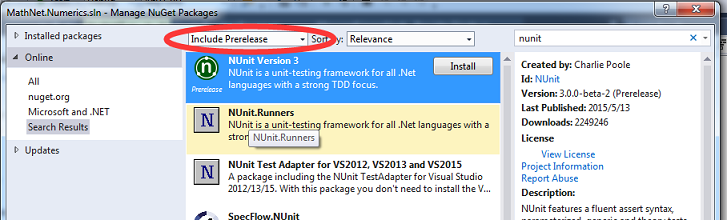
\includegraphics[width=6in]{download_nunit}
	\caption{Downloading Nunit 3.0}
	\label{download_nunit}
\end{figure}

\begin{figure}
	\centering
	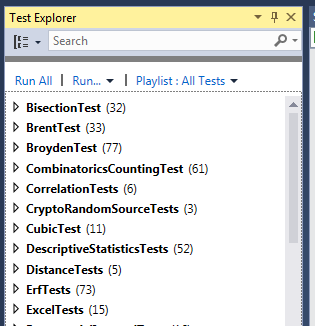
\includegraphics[width=3in]{test_explorer}
	\caption{Test Explorer}
	\label{test_explorer}
\end{figure}

\section{UnitFL as A Coverage Tool}
To collect coverage, you need to open the UnitFL result window from View $->$ Other Windows $->$ UnitFL Result (see Fig~\ref{open_result}).
You need to toggle a button to enable profiling (see Fig~\ref{enable_profiling}). Now UnitFL will collect coverage information for tests. 
Collecting coverage costs a significant overhead, so you should toggle the button again to disable profiling when you don't need coverage.

\begin{figure}
	\centering
	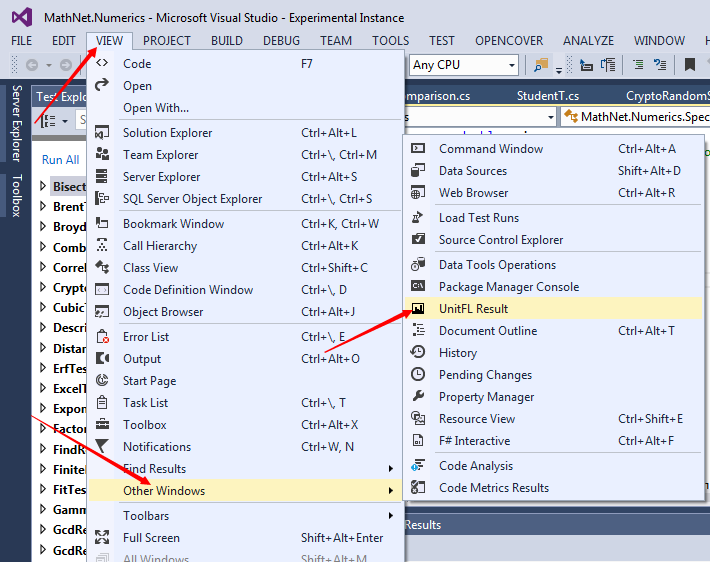
\includegraphics[width=6in]{open_result}
	\caption{Open Result Window}
	\label{open_result}
\end{figure}

\begin{figure}
	\centering
	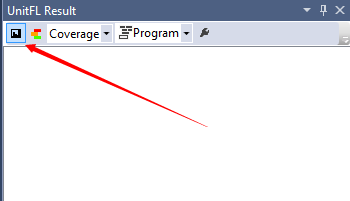
\includegraphics[width=3in]{enable_profiling}
	\caption{Enable Profiling}
	\label{enable_profiling}
\end{figure}

After running tests, coverage information will be displayed in the result window (see Fig~\ref{coverage_result}). In the result window, you can click on a 
class or a method to navigate to the corresponding source code.

\begin{figure}
	\centering
	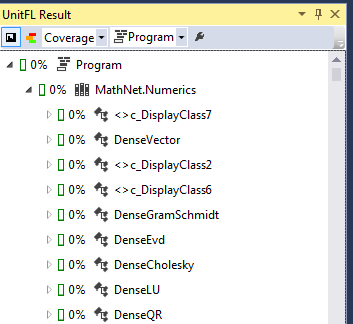
\includegraphics[width=3in]{coverage_result}
	\caption{Coverage Result}
	\label{coverage_result}
\end{figure}

You can toggle a button to enable the coloration of the source code (see Fig~\ref{enable_coloration}). Uncovered lines will be marked red and covered lines will be marked green.

\begin{figure}
	\centering
	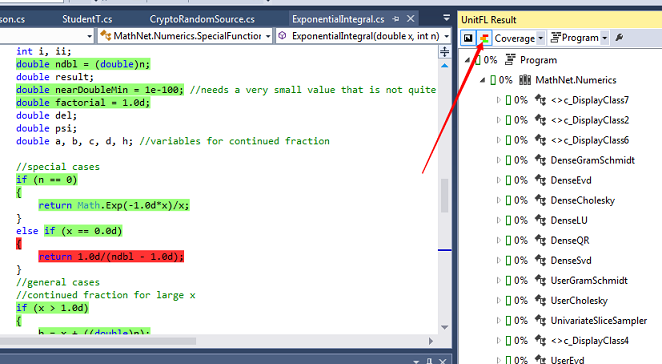
\includegraphics[width=6in]{enable_coloration}
	\caption{Enable Coloration}
	\label{enable_coloration}
\end{figure}

\section{UnitFL as A Fault Localization Tool}
UnitFL can use test reuslts and coverage information to locate faults. To locate fault, you need to enable profiling first and
change the combobox from Coverage to Fault Localization (see Fig~\ref{fault_localization}).

\begin{figure}
	\centering
	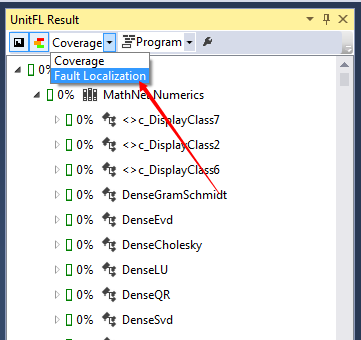
\includegraphics[width=3in]{fault_localization}
	\caption{Fault Localization}
	\label{fault_localization}
\end{figure}

After some of the tests failed, UnitFL will calculate the suspiciousness of every program entity and rank them in the result window (see Fig~\ref{fault_localization_result}).
There are five levels of suspiciousness and they are colored from red to green. Again you can navigate to the source code by click an item and you can toggle the coloration button
to enable coloration of source code.

\begin{figure}
	\centering
	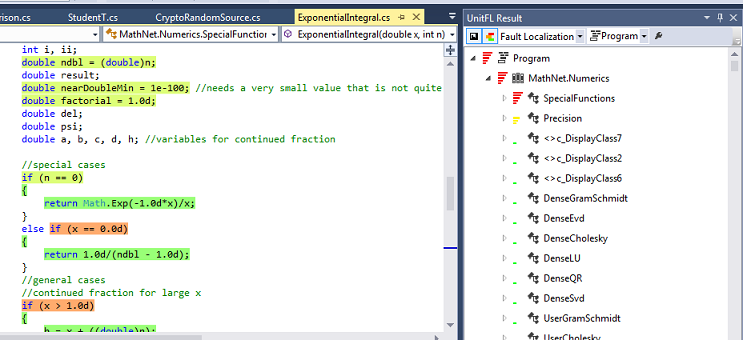
\includegraphics[width=6in]{fault_localization_result}
	\caption{Fault Localization Result}
	\label{fault_localization_result}
\end{figure}

\section{Filters}
You can avoid the profiling some of your assemblies or classes using filters. Filters in UnitFL are very similar to those in OpenCover.
Here are some examples: 
\begin{itemize}
\item{+[*]*, -[*Tests]*} \\
Exclude those assemblies that end with Tests.

\item{+[*Sample]*} \\
Only include those assemblies that end with Sample.

\item{+[*]*, -[*]*Test} \\
Exclude those classes that end with Test.

\end{itemize}

\section{Contact Us}
If you have anything to say, please send a email to wangnangg@gmail.com.


\end{document}
